%% Knowledge-Based Systems short communication (ISSN 0950-7051)
%% Elsevier elsarticle, numbered citations (journal style applied at proof).
%% Compile: pdflatex paper.tex && pdflatex paper.tex
\documentclass[preprint,12pt,3p]{elsarticle}

\usepackage[T1]{fontenc}
\usepackage[utf8]{inputenc}
\usepackage{lmodern}
\usepackage{amsmath,amssymb,amsfonts}
\usepackage{graphicx}
\usepackage{booktabs}
\usepackage{tabularx}
\usepackage{algorithm}
\usepackage{algpseudocode}
\usepackage{xcolor}
\usepackage{xurl}
\usepackage[colorlinks,citecolor=blue,linkcolor=blue,urlcolor=blue]{hyperref}
\usepackage[nameinlink,capitalise,noabbrev]{cleveref}

\journal{Knowledge-Based Systems}

\biboptions{sort&compress}

\graphicspath{{figures/}}

%% Short-communication running head
\DeclareMathOperator{\clip}{clip}

\begin{document}
\begin{frontmatter}

\title{Temporal Knowledge-Graph Features for Firm-Specific Technology Opportunity Prediction}

\author{Eeshwar\corref{cor1}}
\ead{eeshwar.business@gmail.com}
\cortext[cor1]{Corresponding author.}
\affiliation{organization={Independent Researcher}}

\begin{abstract}
Firms that pursue digital innovation must decide which technology domains to explore beyond their current patent portfolios. Graph-based opportunity discovery can look effective when future firm--technology relations leak into features, candidate sets, or random splits. This short communication tests whether temporally valid, inspectable knowledge-graph features improve out-of-time prediction of a firm's first entry into a previously unadopted Cooperative Patent Classification (CPC) subclass. A firm--technology graph is built from public USPTO PatentsView records. Conventional firm and class activity features are compared with the same features plus common-neighbour, co-occurrence, and historical peer-adoption signals. Logistic regression and random forests are trained on identical candidates under chronological evaluation with an embargo year, imbalance-aware metrics, and a firm-clustered bootstrap. On 10{,}878 organization assignees (grant years 2010--2023), the graph-feature forest improved average precision versus the same-learner forest on 2021--2022 pairs (paired 95\% interval 0.015 to 0.019). Absolute average precision remained low against a 1.11\% positive rate, and logistic regression was a competitive ranking baseline. Relational features therefore add incremental signal, but they do not make technology-entry prediction easy or automatically decision-ready.
\end{abstract}

\begin{keyword}
knowledge graph \sep technology opportunity \sep patent analytics \sep temporal validation \sep decision support \sep explainable AI \sep link prediction
\end{keyword}

\end{frontmatter}

\section*{Highlights}
\begin{itemize}
\item Temporally valid graph features are tested for firm technology-entry.
\item A many-firm PatentsView holdout uses an embargoed chronological split.
\item Graph features lift forest AP; logistic regression remains competitive.
\item Absolute AP stays low against a 1.11\% positive technology-entry rate.
\item Relational scores are inspectable inputs, not mandates to enter a class.
\end{itemize}

\noindent\textit{Article type:} Short communication (no more than 10 double-spaced pages, including tables and figures). Upload the five highlight bullets as a separate editable file at submission.

\section{Introduction}
\label{sec:intro}
Digital innovation often requires a firm to move into technology classes that are absent from its current patent portfolio. The firm's own history is an incomplete map: classes co-occur across assignees, peers adopt neighbouring technologies, and those relations change over time. A knowledge-based decision-support system can make those relations explicit, but only if the representation used at prediction time could actually have been observed then.

Firm-specific technology opportunity discovery (TOD) already uses patent graphs and link prediction. F-term co-occurrence networks, graph-convolutional convergence models, heterogeneous assignee--inventor--technology ecologies, and rule-based portfolio graphs have all been used to propose new classes, terms, or patents for a target firm~\cite{lee2021,park2022,choi2023,seol2023,wu2023,wu2026,zhao2025}. Related work searches knowledge networks and hierarchical semantic graphs for opportunities that are not yet covered by any single patent~\cite{liu2023techno,ren2021}, or predicts converging knowledge flows in citation networks~\cite{park2018}. Patent-portfolio and co-classification studies similarly treat opportunity discovery as a mapping from a firm's existing codes to adjacent fields~\cite{shi2019,wang2018su,feng2020,yi2025}. Machine-learning link prediction has also been used to move from opportunity lists to candidate solutions and to forecast previously unconnected classification pairs~\cite{wang2024aei,geum2020,liu2023tfsc,zhao2026}. Topology-based patent recommendation with subject--action--object embeddings provides a firm-specific ranking analogue in the engineering-management literature~\cite{liu2025ieee}.

The existence of a graph is not, by itself, a novelty claim for \emph{Knowledge-Based Systems}. Knowledge-graph and graph-embedding surveys distinguish representation, acquisition, relational scoring, and downstream use~\cite{wang2017ieee,ji2022,nickel2016,cai2018,goyal2018}. Explainable knowledge-graph recommenders further show that inspectable relations can support ranking, but only when the knowledge layer is isolated and evaluated~\cite{yang2020,shimizu2022}. In innovation forecasting the corresponding evaluation failure mode is temporal leakage: future classifications, future firm--class edges, or labels that would not yet have been observable can make a retrospective model look stronger than a deployable one.

This paper therefore asks a narrower, falsifiable question. When candidate technologies, feature timestamps, and evaluation cutoffs are controlled, do compact relational features add out-of-time value over strong tabular baselines? The contribution is a many-firm, leakage-aware technology-entry benchmark on public PatentsView records~\cite{uspto2025,uspto2026}, not a new graph neural network and not a claim that patenting equals innovation. Three hypotheses are pre-specified:
\begin{itemize}
\item \textbf{H1 (incremental value):} the graph-feature model achieves higher average precision than the strongest tabular baseline on the held-out future period.
\item \textbf{H2 (relational contribution):} removing graph-derived features reduces performance relative to the full model when the learner is held constant.
\item \textbf{H3 (temporal robustness):} any improvement is directionally stable across more than one chronological cutoff.
\end{itemize}
H1 is interpreted against the best tabular model on average precision. H2 is the pre-specified same-learner contrast (graph-feature random forest versus tabular random forest). H3 requires a second cutoff; only the protocol's single split is executed here.

\section{Data and knowledge representation}
\label{sec:data}

\subsection{PatentsView extract}
The source is the USPTO PatentsView granted-patent metadata dump covering records through 31 December 2024, archived on Zenodo~\cite{uspto2025}. Later PatentsView files are hosted on the USPTO Open Data Portal~\cite{uspto2026} behind authenticated access; this study therefore uses the last fully public dump. Files \texttt{g\_patent.tsv.zip}, \texttt{g\_assignee\_disambiguated.tsv.zip}, and \texttt{g\_cpc\_current.tsv.zip} were downloaded on 23 October 2026 and joined on \texttt{patent\_id}. Provenance, hashes, and inclusion rules are stored with the normalized extract.

Normalization produces one unique row per firm--year--CPC subclass. The firm identifier is the PatentsView disambiguated \texttt{assignee\_id}. Only assignees with a non-empty organization name are retained. Year is the grant year. Withdrawn patents and non-utility grants are excluded. CPC subclass codes are the first four alphanumeric characters of \texttt{cpc\_subclass}; former-USPC indexing subclasses \texttt{Y10*} are dropped. Joint assignees create multiple firm--technology rows. Firms must have at least eight distinct grant years, eight distinct subclasses, twenty firm--year--CPC rows, and at least one G or H subclass in 2010--2023. After these filters the extract contains 1{,}453{,}416 rows, 10{,}878 firms, 14 years, and 668 subclasses.

Patent-based class entry is a proxy, not a measure of commercial success, non-patented innovation, or digital-transformation adoption. The target below is therefore \textbf{first observed CPC-subclass entry in granted patents}.

\subsection{Unit of analysis and graph}
Let $F$ be the set of firms and $C$ the candidate CPC subclasses. For prediction year $t$, the time-indexed knowledge graph is
\begin{equation}
G_t = (F, C, E_t),\qquad
E_t = \bigl\{(f,c)\in F\times C:\ \text{firm } f \text{ has class } c \text{ in a grant year }\le t\bigr\}.
\label{eq:graph}
\end{equation}
Technology--technology relations are induced from co-occurrence in portfolios observed by $t$. Future edges are not used to score a prediction made at $t$. The candidate universe $C$ is the 30 most frequent subclasses in the 2010--2012 burn-in window and is then held fixed. The design estimates entry into classes already visible in that window; it does not claim to predict entirely unseen subclasses.

The unit of analysis is a firm--candidate--year triple $(f,c,t)$ with $c\notin P_{f,t}$, where $P_{f,t}$ is the set of classes observed for $f$ by the end of year $t$. The binary target is first entry in the following year:
\begin{equation}
y_{f,c,t} = \mathbf{1}\bigl[c \notin P_{f,t}\ \text{and}\ c \in P_{f,t+1}\bigr].
\label{eq:target}
\end{equation}
Eligible prediction years are 2013--2022. Training uses 2013--2019, 2020 is embargoed, and 2021--2022 form the test window. Every feature for $(f,c,t)$ is computed from records dated $\le t$.

\subsection{Feature blocks}
Two feature blocks are used. The conventional block describes firm history and class activity:
\begin{align}
x^{\mathrm{size}}_{f,t} &= |P_{f,t}|,
\label{eq:size}\\
x^{\mathrm{act}}_{f,t} &= \text{number of firm--year--class rows for } f \text{ with year }\le t,
\label{eq:act}\\
x^{\mathrm{prev}}_{c,t} &= n_{c,t}/|F_t|,
\label{eq:prev}\\
x^{\mathrm{gr}}_{c,t} &= \clip\bigl((n^{\mathrm{rec}}_{c,t}-n^{\mathrm{pri}}_{c,t})/\max(1,n^{\mathrm{pri}}_{c,t}),\,-5,5\bigr).
\label{eq:gr}
\end{align}
Here $n_{c,t}$ is the number of firms with class $c$ by year $t$, $F_t$ is the set of firms with any history by $t$, $n^{\mathrm{rec}}_{c,t}$ counts firms active in $c$ in years $\{t-1,t\}$, and $n^{\mathrm{pri}}_{c,t}$ counts firms active in $c$ in years $\{t-3,t-2\}$.

The graph block is intentionally inspectable. Let $\omega_t(c,c')$ be the number of historical portfolios in $G_t$ that contain both $c$ and $c'$, and let $\mathrm{peers}_{f,t}$ be other firms that share at least one class with $f$ by year $t$. Then
\begin{align}
x^{\mathrm{cn}}_{f,c,t} &= \sum_{c'\in P_{f,t}}\omega_t(c,c'),
\label{eq:cn}\\
x^{\mathrm{peer}}_{f,c,t} &= \bigl|\{p\in\mathrm{peers}_{f,t}: c\in P_{p,t}\}\bigr|/\max\bigl(1,|\mathrm{peers}_{f,t}|\bigr),
\label{eq:peer}\\
x^{\mathrm{deg}}_{c,t} &= \bigl|\{c'\in C: \omega_t(c,c')>0\}\bigr|.
\label{eq:deg}
\end{align}
Common-neighbour strength $x^{\mathrm{cn}}$ is a weighted overlap between the firm's portfolio and the candidate. Peer prevalence $x^{\mathrm{peer}}$ is the historical adoption rate among technological neighbours. Degree $x^{\mathrm{deg}}$ is the candidate's co-occurrence connectivity. No graph neural network is trained.

\begin{algorithm}[t]
\caption{Leakage-aware feature construction at prediction year $t$}
\label{alg:features}
\begin{algorithmic}[1]
\Require firm--year--CPC records with grant year $\le t$; fixed candidate set $C$
\Ensure feature vectors for eligible pairs $(f,c)$
\State Build portfolios $P_{f,t}$ and edge set $E_t$ from records dated $\le t$.
\State Count co-occurrence weights $\omega_t(c,c')$ inside those portfolios.
\State Compute class prevalence and clipped recent growth from years $\le t$.
\For{each firm $f$ with $P_{f,t}\neq\emptyset$ and each $c\in C\setminus P_{f,t}$}
    \State Compute the conventional block in Eqs.~\eqref{eq:size}--\eqref{eq:gr} and the graph block in Eqs.~\eqref{eq:cn}--\eqref{eq:deg}.
    \State Set $y_{f,c,t}$ from the firm's classes in year $t+1$ (never used as a feature).
\EndFor
\State \Return the pair panel for year $t$.
\end{algorithmic}
\end{algorithm}

\section{Experimental design}
\label{sec:design}
Three models are compared on the same candidate pairs (\cref{tab:models}):
\begin{enumerate}
\item \textbf{M1}, $\ell_2$-regularized logistic regression with balanced class weights, using only the conventional block.
\item \textbf{M2}, a random forest ($300$ trees, $\sqrt{p}$ features, minimum leaf size $5$, balanced subsample weights), using the same conventional block.
\item \textbf{M3}, the same forest as M2 with the graph block appended.
\end{enumerate}
The primary contrast is M3 versus M2 because it isolates the relational features while holding the learner fixed. M1 is a transparent linear reference. Hyperparameters were fixed before the test window was scored. Numeric preprocessing (median imputation and standardization) is fitted on training rows only. The decision threshold for balanced accuracy is chosen on prediction year 2019, the last training year, by maximizing balanced accuracy on that year; test labels are not used to choose a threshold.

Technology-entry is rare. The primary metric is average precision, always reported with the test positive prevalence. ROC-AUC is secondary because it can look favourable under severe imbalance. Balanced accuracy is reported at the training-year threshold. Brier score is reported for probability quality. For M3 versus M2, a paired bootstrap resamples held-out firms as clusters, retaining all of a firm's test pairs together, and forms a $95\%$ interval for the average-precision difference from $1{,}000$ replicates. H1 is supported only if the graph model beats the strongest tabular baseline on average precision with uncertainty. H2 is supported if the M3--M2 interval excludes no improvement. Multiple cutoffs would be required for H3; they are not used here to select a favourable window.

\section{Results}
\label{sec:results}
Results are taken from the versioned outputs of \texttt{src/experiment.py} on the normalized PatentsView file. Synthetic \texttt{--demo} numbers are not reported.

The candidate universe is the 30 most common CPC subclasses in 2010--2012. Training uses prediction years 2013--2019 ($1{,}540{,}698$ pairs). Year 2020 is embargoed. The test window is 2021--2022 ($455{,}458$ pairs; $10{,}411$ firms; $30$ classes). Test-set positive prevalence is $1.11\%$ ($5{,}057$ first entries). Thresholds were chosen on 2019.

\begin{table}[t]
\centering
\caption{Model comparison and the question each contrast addresses.}
\label{tab:models}
\begin{tabular}{@{}lll@{}}
\toprule
Model & Feature block & Purpose \\
\midrule
M1 logistic regression & Firm history and class activity & Transparent tabular baseline \\
M2 random forest & Same conventional features as M1 & Nonlinear tabular baseline; same learner as M3 \\
M3 graph-feature forest & M2 features plus Eqs.~\eqref{eq:cn}--\eqref{eq:deg} & Incremental value of inspectable graph features \\
\bottomrule
\end{tabular}
\end{table}

\begin{table}[t]
\centering
\caption{Held-out performance on prediction years 2021--2022. Positive prevalence $=0.0111$. Random ranking would yield average precision near that base rate. The paired firm-cluster bootstrap for M3 minus M2 average precision is $\Delta\mathrm{AP}=0.0172$ ($95\%$ interval $0.0155$ to $0.0191$; $1{,}000$ firm clusters).}
\label{tab:results}
\begin{tabular}{@{}lcccc@{}}
\toprule
Model & Average precision & ROC-AUC & Balanced accuracy & Brier score \\
\midrule
M1 logistic & 0.0313 & 0.703 & 0.644 & 0.156 \\
M2 random forest & 0.0155 & 0.597 & 0.573 & 0.046 \\
M3 graph-feature forest & 0.0326 & 0.748 & 0.684 & 0.025 \\
\bottomrule
\end{tabular}
\end{table}

The interval for M3 minus M2 excludes zero, so the pre-specified same-learner comparison supports \textbf{H2}: removing the graph block reduces average precision. M3 also has the best ROC-AUC, balanced accuracy, and Brier score. Absolute average precision remains low for all models ($0.033$ against a $1.11\%$ base rate). \cref{fig:pipeline} records the pipeline used to obtain \cref{tab:results}; \cref{fig:split} records the split.

\textbf{H1 is not supported on the pre-specified reading.} The strongest tabular model on average precision is M1 ($0.0313$), not M2 ($0.0155$). M3's advantage over M1 is $0.0013$ and has no pre-specified cluster interval. Logistic regression is therefore a competitive ranking baseline; the forest without graph features is not. \textbf{H3 is not tested:} only one embargoed cutoff was run.

\begin{figure}[t]
\centering
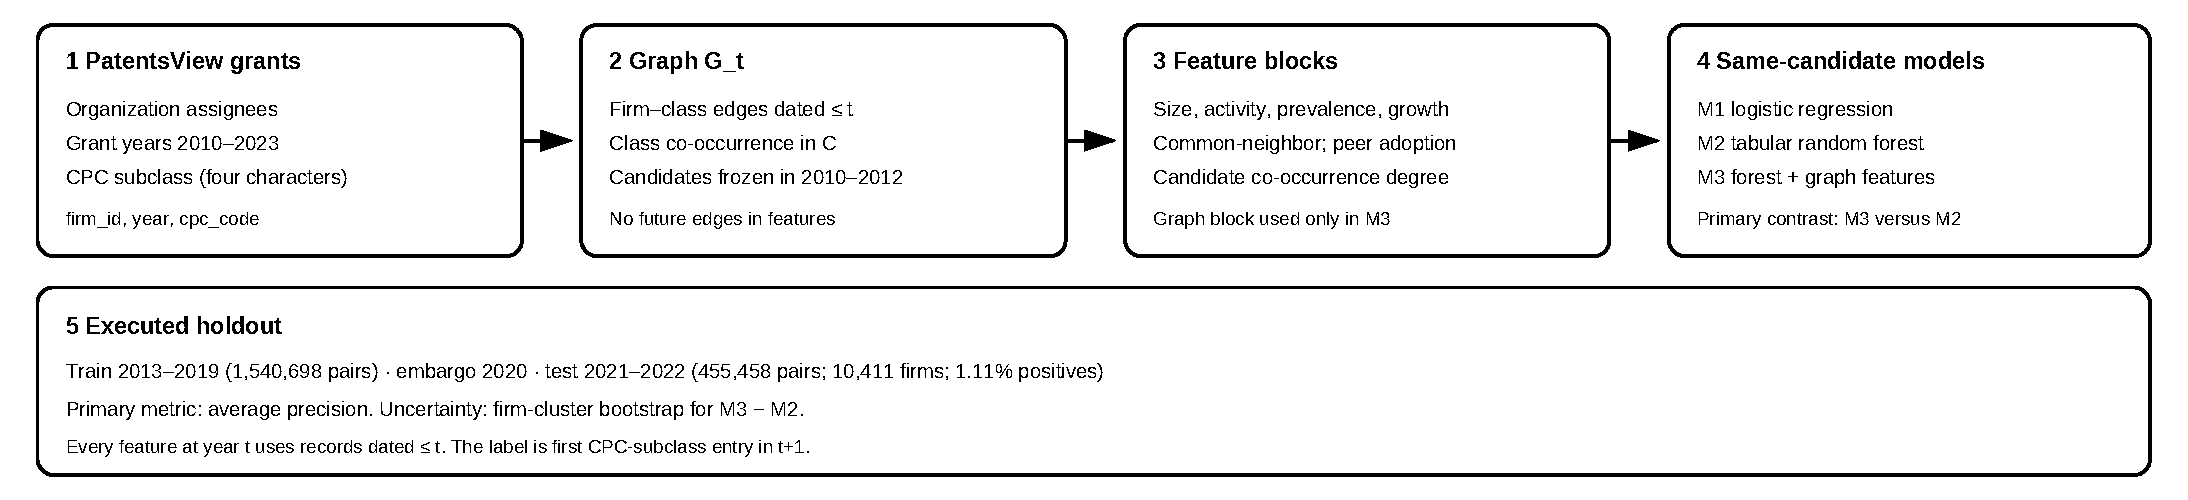
\includegraphics[width=\textwidth]{figure1_architecture.pdf}
\caption{Knowledge-graph feature pipeline. Time-stamped PatentsView relations become the graph $G_t$, inspectable features, and a three-model comparison under one chronological protocol.}
\label{fig:pipeline}
\end{figure}

\begin{figure}[t]
\centering
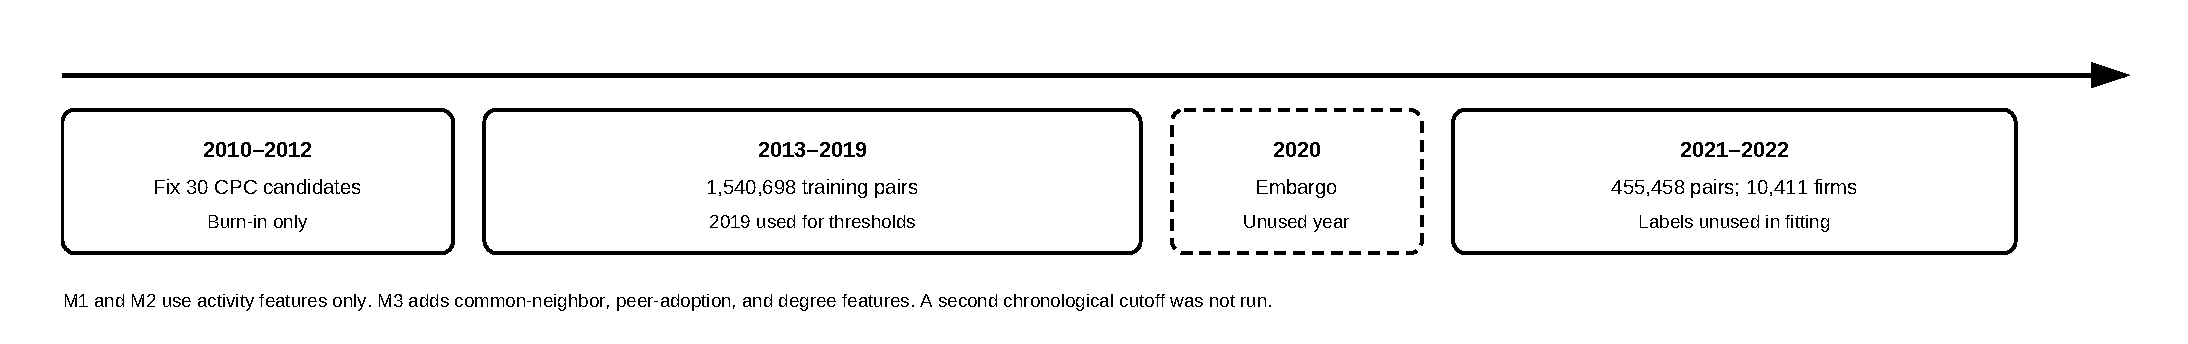
\includegraphics[width=\textwidth]{figure2_evaluation.pdf}
\caption{Executed leakage-aware split. Burn-in years 2010--2012 fix the candidate universe; training uses 2013--2019; 2020 is embargoed; 2021--2022 are scored but never used for fitting. This is a protocol diagram, not a performance chart.}
\label{fig:split}
\end{figure}

\section{Discussion}
\label{sec:discussion}
On this extract, inspectable graph features added average-precision value when the learner was held constant. Co-occurrence, common-neighbour, and peer-adoption signals therefore contain information that the forest does not recover from portfolio size, activity, class prevalence, and recent growth alone. That finding is consistent with TOD studies that treat relational structure as informative~\cite{lee2021,park2022,choi2023,seol2023,wu2023,wu2026,zhao2025,yi2025,liu2025ieee}, but it does not reproduce their typical claim of operational opportunity lists for one focal firm. The many-firm, embargoed protocol is stricter, and the absolute scores are modest.

The result also warns against treating ``nonlinear model'' as a substitute for a linear baseline. M1 matched M3 closely on average precision and beat M2 by a wide margin. Class-weighted logistic regression, however, had a much worse Brier score than either forest, so its scores should not be read as frequencies. For decision support, ranking and calibration must be reported together~\cite{yang2020,shimizu2022}.

The practical implication is bounded. Average precision of $0.033$ against a $1.11\%$ base rate is better than random ranking, but most highly scored firm--class pairs will still not enter next year. The system can prioritize review lists; it cannot authorize entry. Opportunity ranking remains an input to strategy, cost, regulation, capability, and demand, none of which are in the target~\cite{shi2019,feng2020}. The knowledge layer here is a small, auditable feature block rather than an opaque embedding, which is the representation style advocated by graph-embedding and knowledge-graph surveys when explanations are required~\cite{wang2017ieee,ji2022,nickel2016,cai2018,goyal2018}.

The contribution is therefore not another GNN case study~\cite{park2022,wu2026,liu2023techno}. It is a compact test of whether a relational block earns its place next to standard activity features when leakage is controlled. H3 remains open; M3 versus M1 was not the pre-specified bootstrap contrast; grant year is not application year; and CPC revisions are not concorded.

Limitations follow from the design. Assignee disambiguation and grant timing introduce measurement error~\cite{uspto2025,uspto2026}. The fixed candidate universe excludes classes absent from 2010--2012. Graph features may favour patent-intensive firms, and holdout performance can deteriorate under drift. Model scores should not be used to deny funding or to make high-stakes decisions without independent validation and human review.

\section{Conclusion}
\label{sec:conclusion}
This short communication tests whether temporal knowledge-graph features improve firm-specific technology-entry prediction over conventional models. On USPTO PatentsView organization assignees from 2010--2023, graph features improved the random forest on a 2021--2022 holdout, with a firm-clustered interval that excluded no gain. Logistic regression remained a strong ranking baseline, and absolute average precision stayed low. Relational features therefore earn a place in this decision-support stack only as incremental, inspectable signals---not as a claim of easy or causal opportunity discovery.

\section*{CRediT authorship contribution statement}
\textbf{Eeshwar:} Conceptualization, Methodology, Software, Formal analysis, Data curation, Writing -- original draft, Writing -- review and editing.

\section*{Declaration of competing interest}
The author declares that there are no known competing financial interests or personal relationships that could have appeared to influence the work reported in this paper.

\section*{Funding}
This research did not receive any specific grant from funding agencies in the public, commercial, or not-for-profit sectors.

\section*{Declaration of generative AI and AI-assisted technologies in the manuscript preparation process}
During the preparation of this work the author used Cursor-hosted AI tools to support literature metadata checking, manuscript language editing, and code documentation. After using these tools, the author reviewed and edited the content as needed and takes full responsibility for the content of the published article. The tools were not used to generate primary experimental images or to invent sources, data, or results.

\section*{Data availability}
The PatentsView granted-patent metadata used in this study are available from Zenodo~\cite{uspto2025}. The normalized \texttt{firm\_id,year,cpc\_code} extract, provenance file, preparation script, experiment code, and measured outputs are in the accompanying repository: \url{https://github.com/eeshwar-research/research-paper}. Raw TSV dumps are reproduced with \texttt{src/prepare\_patentsview.py} and are not stored in git.

\section*{Acknowledgements}
The author thanks the USPTO PatentsView programme for publishing disambiguated patent metadata.

\begin{thebibliography}{00}

\bibitem{lee2021}
J. Lee, N. Ko, J. Yoon, C. Son, An approach for discovering firm-specific technology opportunities: Application of link prediction to F-term networks, Technol. Forecast. Soc. Change 168 (2021) 120746. \url{https://doi.org/10.1016/j.techfore.2021.120746}.

\bibitem{park2022}
M. Park, Y. Geum, Two-stage technology opportunity discovery for firm-level decision making: GCN-based link-prediction approach, Technol. Forecast. Soc. Change 183 (2022) 121934. \url{https://doi.org/10.1016/j.techfore.2022.121934}.

\bibitem{choi2023}
J. Choi, C. Lee, J. Yoon, Exploring a technology ecology for technology opportunity discovery: A link prediction approach using heterogeneous knowledge graphs, Technol. Forecast. Soc. Change 186 (2023) 122161. \url{https://doi.org/10.1016/j.techfore.2022.122161}.

\bibitem{seol2023}
Y. Seol, S. Lee, C. Kim, J. Yoon, J. Choi, Towards firm-specific technology opportunities: A rule-based machine learning approach to technology portfolio analysis, J. Informetr. 17~(4) (2023) 101464. \url{https://doi.org/10.1016/j.joi.2023.101464}.

\bibitem{wu2023}
Y. Wu, Y. Ji, Identifying firm-specific technology opportunities from the perspective of competitors by using association rule mining, J. Informetr. 17~(2) (2023) 101398. \url{https://doi.org/10.1016/j.joi.2023.101398}.

\bibitem{wu2026}
Y. Wu, Z. Lin, Y. Ji, F. Gu, Identifying firm-specific technology opportunities: Heterogeneous graph neural network-based link prediction, Technovation 151 (2026) 103405. \url{https://doi.org/10.1016/j.technovation.2025.103405}.

\bibitem{zhao2025}
R. Zhao, W. Wei, Z. Zhu, Discovering firm technology opportunities by machine learning prediction method based on firm's technology portfolio, Technol. Forecast. Soc. Change 221 (2025) 124305. \url{https://doi.org/10.1016/j.techfore.2025.124305}.

\bibitem{liu2023techno}
Z. Liu, J. Feng, L. Uden, Technology opportunity analysis using hierarchical semantic networks and dual link prediction, Technovation 128 (2023) 102872. \url{https://doi.org/10.1016/j.technovation.2023.102872}.

\bibitem{ren2021}
H. Ren, Y. Zhao, Technology opportunity discovery based on constructing, evaluating, and searching knowledge networks, Technovation 101 (2021) 102196. \url{https://doi.org/10.1016/j.technovation.2020.102196}.

\bibitem{park2018}
I. Park, B. Yoon, Technological opportunity discovery for technological convergence based on the prediction of technology knowledge flow in a citation network, J. Informetr. 12~(4) (2018) 1199--1222. \url{https://doi.org/10.1016/j.joi.2018.09.007}.

\bibitem{shi2019}
X. Shi, L. Cai, H. Song, Discovering potential technology opportunities for fuel cell vehicle firms: A multi-level patent portfolio-based approach, Sustainability 11~(22) (2019) 6381. \url{https://doi.org/10.3390/su11226381}.

\bibitem{wang2018su}
H.C. Wang, Y.C. Chi, P.L. Hsin, Constructing patent maps using text mining to sustainably detect potential technological opportunities, Sustainability 10~(10) (2018) 3729. \url{https://doi.org/10.3390/su10103729}.

\bibitem{feng2020}
L. Feng, Y. Niu, Z. Liu, J. Wang, K. Zhang, Discovering technology opportunity by keyword-based patent analysis: A hybrid approach of morphology analysis and USIT, Sustainability 12~(1) (2020) 136. \url{https://doi.org/10.3390/su12010136}.

\bibitem{yi2025}
S.K. Yi, C.H. Song, A dual-level prediction approach for uncovering technology convergence opportunities: The case of electric vehicles, Sustainability 17~(8) (2025) 3607. \url{https://doi.org/10.3390/su17083607}.

\bibitem{wang2024aei}
Z. Wang, W. Guo, H. Shao, L. Wang, Z. Chang, Y. Zhang, From technology opportunities to solutions generation via patent analysis: Application of machine learning-based link prediction, Adv. Eng. Inform. 62 (2024) 102944. \url{https://doi.org/10.1016/j.aei.2024.102944}.

\bibitem{geum2020}
Y. Geum, M. Kim, How to identify promising chances for technological innovation: Keygraph-based patent analysis, Adv. Eng. Inform. 46 (2020) 101155. \url{https://doi.org/10.1016/j.aei.2020.101155}.

\bibitem{liu2023tfsc}
Z. Liu, J. Feng, L. Uden, From technology opportunities to ideas generation via cross-cutting patent analysis: Application of generative topographic mapping and link prediction, Technol. Forecast. Soc. Change 192 (2023) 122565. \url{https://doi.org/10.1016/j.techfore.2023.122565}.

\bibitem{zhao2026}
J. Zhao, J. Li, X. Xi, W. Liu, Embracing technological opportunities based on heterogeneous networks: An integrated link prediction approach for technology convergence of firms, Technol. Forecast. Soc. Change 229 (2026) 124701. \url{https://doi.org/10.1016/j.techfore.2026.124701}.

\bibitem{liu2025ieee}
Z. Liu, X. Wang, J. Feng, Firm-specific patent recommendation using topology-based link prediction and SAO embedding method, IEEE Trans. Eng. Manag. 72 (2025) 2097--2115. \url{https://doi.org/10.1109/TEM.2025.3570659}.

\bibitem{wang2017ieee}
Q. Wang, Z. Mao, B. Wang, L. Guo, Knowledge graph embedding: A survey of approaches and applications, IEEE Trans. Knowl. Data Eng. 29~(12) (2017) 2724--2743. \url{https://doi.org/10.1109/TKDE.2017.2754499}.

\bibitem{ji2022}
S. Ji, S. Pan, E. Cambria, P. Marttinen, P.S. Yu, A survey on knowledge graphs: Representation, acquisition, and applications, IEEE Trans. Neural Netw. Learn. Syst. 33~(2) (2022) 494--514. \url{https://doi.org/10.1109/TNNLS.2021.3070843}.

\bibitem{nickel2016}
M. Nickel, K. Murphy, V. Tresp, E. Gabrilovich, A review of relational machine learning for knowledge graphs, Proc. IEEE 104~(1) (2016) 11--33. \url{https://doi.org/10.1109/JPROC.2015.2483592}.

\bibitem{cai2018}
H. Cai, V.W. Zheng, K.C.-C. Chang, A comprehensive survey of graph embedding: Problems, techniques, and applications, IEEE Trans. Knowl. Data Eng. 30~(9) (2018) 1616--1637. \url{https://doi.org/10.1109/TKDE.2018.2807452}.

\bibitem{goyal2018}
P. Goyal, E. Ferrara, Graph embedding techniques, applications, and performance: A survey, Knowl.-Based Syst. 151 (2018) 78--94. \url{https://doi.org/10.1016/j.knosys.2018.03.022}.

\bibitem{yang2020}
Z. Yang, S. Dong, {HAGERec}: Hierarchical attention graph convolutional network incorporating knowledge graph for explainable recommendation, Knowl.-Based Syst. 204 (2020) 106194. \url{https://doi.org/10.1016/j.knosys.2020.106194}.

\bibitem{shimizu2022}
R. Shimizu, M. Matsutani, M. Goto, An explainable recommendation framework based on an improved knowledge graph attention network with massive volumes of side information, Knowl.-Based Syst. 239 (2022) 107970. \url{https://doi.org/10.1016/j.knosys.2021.107970}.

\bibitem{uspto2025}
United States Patent and Trademark Office, Final release of PatentsView metadata, pre-grant and granted (12/31/2024) [dataset], Zenodo, 2025. \url{https://doi.org/10.5281/zenodo.15058362}.

\bibitem{uspto2026}
United States Patent and Trademark Office, PatentsView: Research-ready patent data and data downloads, 2026. \url{https://www.uspto.gov/ip-policy/economic-research/patentsview} (accessed 23 October 2026).

\end{thebibliography}

\end{document}
